\documentclass[a4paper, 11pt]{article}
\usepackage[russian]{babel}
\usepackage{ textcomp }
\usepackage[a4paper, total={170mm,257mm}, left=20mm, right=20mm, top=15mm, bottom=15mm]{geometry}
\usepackage[utf8]{inputenc}
\usepackage{graphicx}
\usepackage{amsthm}
\usepackage{amsmath}
\usepackage{tabularx}
\usepackage{amsfonts}
\usepackage{amssymb}
\usepackage{subcaption}
\usepackage{floatflt}
\usepackage{graphicx}
\usepackage[unicode, pdftex]{hyperref}
\usepackage{tikz}
\usetikzlibrary{shapes.geometric}
\usetikzlibrary{decorations.markings}
\usetikzlibrary{calc}
\usetikzlibrary{intersections}
\usepackage{caption}  % in preamble
\usepackage{fancyhdr}
\pagestyle{fancy}
\usepackage{listings}

\usetikzlibrary{decorations,decorations.pathmorphing,decorations.pathreplacing}
\usepackage{tkz-euclide}
\tikzset{%
	add/.style args={#1 and #2}{
		to path={%
			($(\tikztostart)!-#1!(\tikztotarget)$)--($(\tikztotarget)!-#2!(\tikztostart)$)%
			\tikztonodes},add/.default={.2 and .2}}
}  

\usepackage{ gensymb }

\makeatletter
\pgfmathdeclarefunction{distance}{2}{%
	\begingroup%
	\pgfextractx{\pgf@xa}{\pgfpointanchor{#1}{center}}%
	\pgfextracty{\pgf@ya}{\pgfpointanchor{#1}{center}}%
	\pgfextractx{\pgf@xb}{\pgfpointanchor{#2}{center}}%
	\pgfextracty{\pgf@yb}{\pgfpointanchor{#2}{center}}%
	\pgfmathparse{veclen(\pgf@xa-\pgf@xb,\pgf@ya-\pgf@yb)}%
	\pgfmathsmuggle\pgfmathresult\endgroup%
}
\renewcommand{\theenumi}{(\asbuk{enumi})}
\renewcommand{\labelenumi}{\asbuk{enumi})}

\DeclareMathOperator{\sign}{sign}
\DeclareMathOperator{\atan2}{atan2}


\pagestyle{fancy}
\fancyhead[R]{Математический анализ 1 курс}
\fancyhead[L]{2021-2022 год}

\newcommand*{\titlePage}{
	\thispagestyle{empty}
	\begingroup
	\begin{center}
		{\footnotesize
			Министерство образования и науки Российской Федерации\\
			Федеральное государственное автономное образовательное учреждение высшего образования
		}
		
		\vspace*{6ex}
		
		{\large
			САНКТ-ПЕТЕРБУРГСКИЙ НАЦИОНАЛЬНЫЙ ИССЛЕДОВАТЕЛЬСКИЙ УНИВЕРСИТЕТ ИНФОРМАЦИОННЫХ ТЕХНОЛОГИЙ, МЕХАНИКИ И ОПТИКИ	
		}
		
		\vspace*{2ex}
		
		{\large
			Факультет систем управления и робототехники
		}
		
		\vspace*{15ex}
		
		{\LARGE \bfseries 
			Лабораторная работа №1\\
			"Интеграл Римана"\\
			по дисциплине "Математический анализ"\\
		}
		\vspace*{2ex}
		{\Large \itshape
			Вариант 14 \\
			$f(x) = x^3, \quad [0,\,2]$
		}
	\end{center}
	\vspace*{20ex}
	\begin{flushright}
		{\Large 
			\underline{Выполнил}: студент гр. \textbf{R3138}\\
			\begin{flushright}
				Магазенков Е. Н.\\
			\end{flushright}
		}
		
		\vspace*{5ex}
		
		{\Large 
			\underline{Преподаватели}: Бойцев А. А.,\\
			доцент фак. СУиР \\
			Попов А. ,\\
			хороший человек фак. СУиР
		}
	\end{flushright}	
	
	\vspace*{30ex}
	\begin{center}
		{\large 
			Санкт-Петербург, 2022
		}
	\end{center}
	\endgroup}


\begin{document}
	
	\titlePage
	\newpage
	\section{Теоретическое вычисление интеграла}
	\subsection{Существование интеграла Римана}
	Функция $f(x) = x^3$ является непрерывной на отрезке $[0,\,2]$, а значит, согласно теореме об интегрируемости непрерывной функции, интегрируема. \\
	Тогда для нахождения значения интеграла можем выбрать любое разбиение. 
	
	\subsection{Вычисление интеграла по определению}
	\subsubsection{Нахождение интегральной суммы}
	Рассмотрим равномерное разбиение $\color{blue} \tau$ отрезка $[0,\, 2]$:
	\begin{equation}
		{\color{blue} x_i} = \frac{2i}{n}
	\end{equation}
	\begin{center}
	\begin{tikzpicture}
		\draw[->] (0,0) -- (14,0) node[right]{$x$};
		\filldraw[red] (1,0) node[below]{$x_0 = 0$} circle(1.5pt);
		\filldraw[red] (13,0) node[below]{$x_n = 2$} circle(1.5pt);
		\foreach \x in {1,2} {
		\filldraw[blue] (2*\x+1, 0) node[below]{$x_{\x} = \frac{2 \cdot \x}{n}$} circle(1pt);
		}
		\filldraw[blue] (11, 0) node[below]{$x_{n-1} = \frac{2 \cdot (n-1)}{n}$} circle(1pt);
		\draw[blue] (8,-0.4) node {$\dots$};
	\end{tikzpicture}
	\end{center}
	Возьмём в качестве оснащения $\color{orange}\xi$ правые границы отрезков:
	\begin{equation}
		\xi_i = x_i = \frac{2i}{n}
	\end{equation}
	\begin{center}
		\begin{tikzpicture}
			\draw[->] (0,0) -- (14,0) node[right]{$x$};
			\filldraw[red] (1,0) node[below]{$x_0 = 0$} circle(1.5pt);
			\filldraw[red] (13,0) node[below]{$x_n = 2$} circle(1.5pt);
			\foreach \x in {1,2} {
				\filldraw[blue] (2*\x+1, 0) node[below]{$x_{\x} = \frac{2 \cdot \x}{n}$} circle(1pt);
				\draw[orange] (2*\x + 1, 0) node[above]{$\xi_\x$}; 
			}
			\filldraw[blue] (11, 0) node[below]{$x_{n-1} = \frac{2 \cdot (n-1)}{n}$} circle(1pt);
			\draw[orange] (11, 0) node[above]{$\xi_{n-1}$}; 
			\draw[orange] (8,0.3) node {$\dots$};
			\draw[blue] (8,-0.4) node {$\dots$};
		\end{tikzpicture}
	\end{center}
	Тогда согласно определению $\sigma_{\tau} (f,\, \xi) = \sum\limits_{i=0}^n f(\xi_i) \cdot \Delta_i$
	\begin{equation}
		\sigma_{\tau} (x^3, \, \xi) = \sum\limits_{i=0}^n \left(\frac{2i}{n}\right)^3 \cdot \frac{2}{n}
	\end{equation}
	\begin{center}
		\begin{tikzpicture}
			\draw[very thin,opacity=0.4, gray] (-0.9, -0.9) grid (7.9,8.9);
			\draw[->] (-1,0) -- (8, 0)node[right]{$x$};
			\draw[->] (0,-1) -- (0, 9)node[above]{$y$};
			\draw[purple, very thick, domain=0:2, smooth] plot(\x, {\x^3});
			\filldraw[red] (0,0) node[below left] {$0$};
			\filldraw[red] (2,0) node[below right] {$2$};
			\foreach \x in {.1, .2, ..., 2}{
				\draw (\x-.1, 0) rectangle (\x, \x^3);	
		}
		\end{tikzpicture}
	\end{center}
	Вычисляя эту сумму, получаем
	\begin{equation*}
		 \sigma_{\tau} (x^3, \, \xi) = \frac{2}{n} \cdot \sum\limits_{i=0}^n \left(\frac{2i}{n}\right)^3 = \frac{2}{n} \cdot \left(\frac{2}{n}\right)^3 \cdot \left(\frac{n \cdot (n+1)}{2}\right)^2 
	\end{equation*}
	\begin{equation}
		 \sigma_{\tau} (x^3, \, \xi) = \frac{4(n+1)^2}{n^2}
	\end{equation}
	\subsubsection{Переход к интегралу Римана}
	Тогда определённый интеграл Римана можно найти используя определение 
	\begin{equation}
		\int\limits_0^2 x^3 \,dx = \lim\limits_{n \to +\infty}  \sigma_{\tau} (x^3, \, \xi)
	\end{equation}
	\begin{equation}
		\int\limits_0^2 x^3 \,dx = \lim\limits_{n \to +\infty}  \frac{4(n+1)^2}{n^2} = 4 \label{by_def}
	\end{equation}
	
	\subsection{Вычисление интеграла по формуле Ньютона-Лейбница}
	Согласно формуле Ньтона-Лейбница $\int\limits_a^b f(x)\, dx = F(a) - F(b)$, где $F(x)$ -- первообразная функция для $f(x)$
	Применяя данную формулу к нашей функции, получаем
	\begin{equation}
		\int\limits_0^2 x^3 \, dx = \left. \frac{x^4}{4} \right|_0^2 = \frac{2^4}{4} - \frac{0^4}{4} = 4 \label{by_NL}
	\end{equation}
	\subsection{Анализ результатов}
	Таким образом, мы вычислили интеграл $\int\limits_0^2 x^3 \, dx$ двумя способами: по определению и с помощью формулы Ньютона-Лейбница.\\
	Сравнив результаты вычислений \ref{by_def} и \ref{by_NL}, понимаем, что они совпадают.
	
	\section{Оценка погрешностей вычислений}
	\subsection{Вывод формулы теоретической погрешности интеграла и его приближения}
	Найдём значение погрешности вычисления интеграла методом прямоугольников
	\begin{equation}
		\left|R_n\right| = \left| \int\limits_a^b f(x) \,dx - \sigma_{\tau}(f, \xi) \right|
	\end{equation}
	Воспользуемся свойством аддитивности интеграла
	\begin{equation}
		\int\limits_a^b f(x) \, dx = \sum_{i=0}^{n} \int\limits_{x_{i}}^{x_{i+1}} f(x) \, dx
	\end{equation}	
	\subsection{Случай оснащения правыми границами отрезков}
	Интегральную сумму при оснащении правыми границами отрезков можно расписать как
	\begin{equation}
		\sigma_{\tau}(f, \xi) = \sum_{i=0}^n f(x_{i+1}) \cdot (x_{i+1}-x_i) = \sum_{i=0}^n \int\limits_{x_{i}}^{x_{i+1}} f(x_{i+1}) \, dx
	\end{equation}
	Тогда можем переписать погрешность интеграла
	\begin{equation}\label{11}
		\left|R_n\right| = \left| \sum_{i=0}^{n} \int\limits_{x_{i}}^{x_{i+1}} f(x) \, dx - \sum_{i=0}^n \int\limits_{x_{i}}^{x_{i+1}} f(x_{i+1}) \, dx \right| = \left| \sum_{i=0}^n \int\limits_{x_{i}}^{x_{i+1}}\left(f(x) - f(x_{i+1})\right) \, dx \right|
	\end{equation}
	Пусть $f(x)$ дифференцируема на отрезке $[a,\,b]$. Распишем функцию $f(x)$ по формуле Тейлора с остатком в форме Лагранжа в точках $x_{i}$
	\begin{equation}\label{key}
		f(x) = f(x_{i}) + f'(\eta_i) \cdot (x-x_{i}), \quad \eta_i \in [x, x_{i}]
	\end{equation}
	Тогда остаток равен
	\begin{equation}\label{key}
		\left|R_n\right| = \left| \sum_{i=0}^n \int_{x_i}^{x_{i+1}} f'(\eta_i) \cdot (x - x_{i})\, dx\right|
	\end{equation}
	Оценим его неравенством треугольника, а затем самым простым способом: $\left|f'(\eta_i)\right| \leqslant \max\limits_{[a,\,b]} \left|f'(x)\right|$
	\begin{equation}\label{14}
		\left|R_n\right| \leqslant \sum_{i=0}^n \int_{x_i}^{x_{i+1}} \left|f'(\eta_i)\right| \cdot (x_{i+1} - x_i)\, dx  \leqslant \sum_{i=0}^n \max\limits_{[a,\,b]} \left|f'(x)\right| \cdot \frac{(x_{i+1} - x_i)^2}{2} 
	\end{equation} 
	Каждую из разностей заменим длиной отрезка $(x_{i+1} - x_i) = \frac{b-a}{n}$
	\begin{equation}\label{15}
		\left|R_n\right| \leqslant \max\limits_{[a,\,b]} \left|f'(x)\right| \cdot n \cdot \frac{\left(\frac{b-a}{n}\right)^2}{2}
	\end{equation}
	Таким образом, 
	\begin{equation}\label{16}
		 \left|R_n\right| \leqslant \max\limits_{[a,\,b]} \left|f'(x)\right| \frac{(b-a)^2}{2n}
	\end{equation}
	\subsection{Случай оснащения центральными точками отрезков}
	Аналогично можно оценить для оснащения центральными точками отрезков $\xi_i = \frac{x_{i+1} + x_i}{2}$
	Подставляя в \ref{11}, получаем
	\begin{equation}\label{key}
		\left|R_n\right| = \left| \sum_{i=0}^n \int\limits_{x_{i}}^{x_{i+1}}\left(f(x) - f\left(\frac{x_{i+1}+x_i}{2}\right)\right) \, dx \right|
	\end{equation}
	Пусть $f(x)$ дважды дифференцируема на отрезке $[a,\,b]$ . Распишем функцию $f(x)$ по формуле Тейлора с остатком в форме Лагранжа в точке $\frac{x_{i+1}-x_i}{2}$.
	\begin{equation}\label{key}
		f(x) = f\left(\frac{x_{i+1} - x_i}{2}\right) + f'\left(\frac{x_{i+1}-x_i}{2}\right) \cdot \left(x - \frac{x_{i+1}-x_i}{2}\right) + \frac{f''\left(\eta_i\right) \cdot \left(x - \frac{x_{i+1}-x_i}{2}\right)^2}{2} 
	\end{equation}
	Тогда остаток 
	\begin{equation}\label{key}
		\left|R_n\right| = \left| \sum_{i=0}^n \int\limits_{x_{i}}^{x_{i+1}} \left( f'\left(\frac{x_{i+1}-x_i}{2}\right) \cdot \left(x - \frac{x_{i+1}-x_i}{2}\right) + \frac{f''\left(\eta_i\right) \cdot \left(x - \frac{x_{i+1}-x_i}{2}\right)^2}{2} \right) \, dx \right|
	\end{equation}
	Вычисляя интеграл, получаем
	\begin{equation}\label{key}
		\left|R_n\right| = \left| \sum_{i=0}^n \left.f'\left(\frac{x_{i+1}-x_i}{2}\right) \cdot \frac{\left(x - \frac{x_{i+1}-x_i}{2}\right)^2}{2} \right|_{x_i}^{x_{i+1}} + \left. \frac{f''\left(\eta_i\right) \cdot \left(x - \frac{x_{i+1}-x_i}{2}\right)^3}{6} \right|_{x_i}^{x_{i+1}} \right|
	\end{equation}
	\begin{equation}\label{key}
		|R_n| = \left| 0 + \frac{f''\left(\eta_i\right) \cdot \left(\frac{x_{i+1}-x_i}{2}\right)^3}{3} \right|
	\end{equation}
	Проводя далее оценку, аналогичную \ref{14} и \ref{15}, получаем
	\begin{equation}\label{22}
		\left|R_n\right| \leqslant \max\limits_{[a,\,b]} \left|f''(x)\right| \frac{(b-a)^3}{24n^2}
	\end{equation}
	\subsection{Применительно к интегралу $\int\limits_0^2 x^3\, dx$}
	Оценим вычисления при использовании центральной точки отрезков разбиения по формуле~\ref{22}
	\begin{equation}\label{key}
		\left|R_n\right| \leqslant \max\limits_{[0,\,2]} \left|(x^3)''\right| \frac{(2-0)^3}{24n^2} = \max\limits_{[0,\,2]} \left|6x\right| \frac{8}{24n^2} = \frac{12\cdot8}{24n^2} = \frac4{n^2}
	\end{equation}
	При использовании крайних точек отрезков оценим по формуле~\ref{16}
	\begin{equation}
		\left|R_n\right| \leqslant \max\limits_{[0,\,2]} \left|(x^3)'\right| \frac{(2-0)^2}{2n} = \max\limits_{[0,\,2]} \left|3x^2\right| \frac{4}{2n} = \frac{12\cdot4}{2n} = \frac{24}{n}
	\end{equation}
	\section{Работа программы}
	Программа для вычисления интеграла, используя метод прямоугольников, написана на языке \itshape{Python3} с использованием библиотеки \itshape{manim}\\
	Результат работы программы можно увидеть на Рис.\ref{result}, а также по  \href{https://github.com/Egor-Magazenkov/Math_analysis_Lab_1}{ссылке}
	\begin{figure}
		\begin{center}
			\begin{subfigure}{0.45\linewidth}
				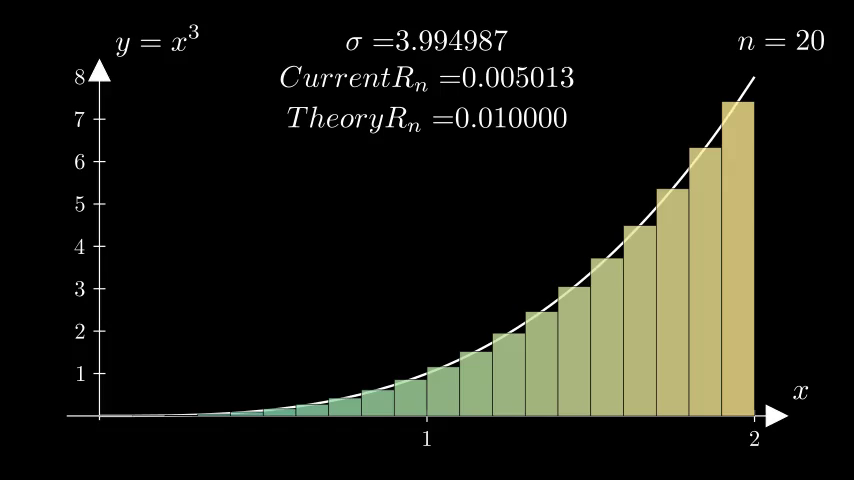
\includegraphics[width=\linewidth]{"./20.png"}
				\caption{при $n=20$}
			\end{subfigure}
			\begin{subfigure}{0.45\linewidth}
				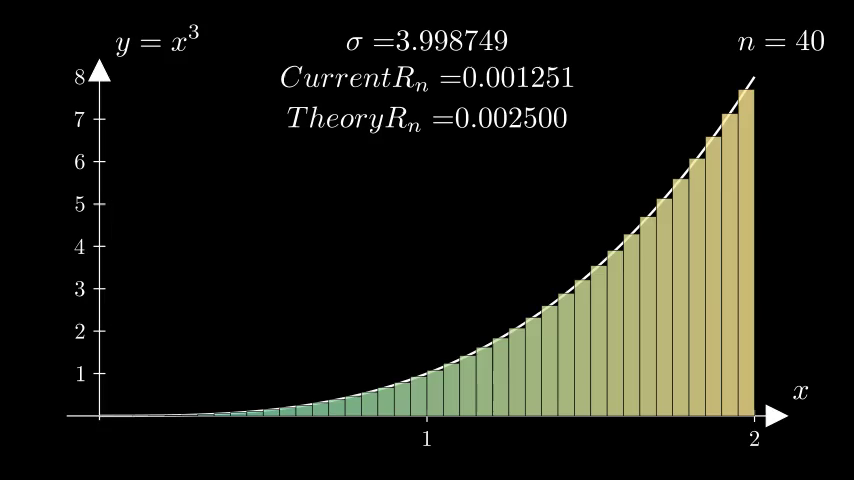
\includegraphics[width=\linewidth]{"./40.png"}
				\caption{при $n=40$}
			\end{subfigure}
			\begin{subfigure}{0.45\linewidth}
				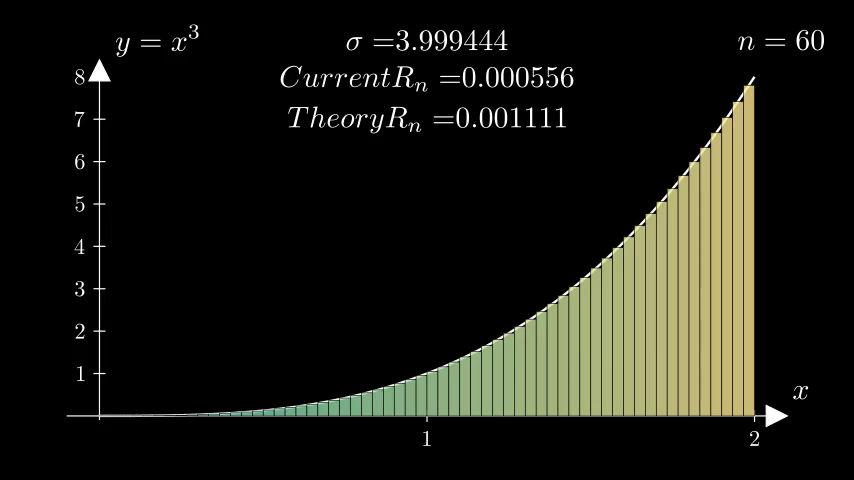
\includegraphics[width=\linewidth]{"./60.png"}
				\caption{при $n=60$}
			\end{subfigure}
			\begin{subfigure}{0.45\linewidth}
				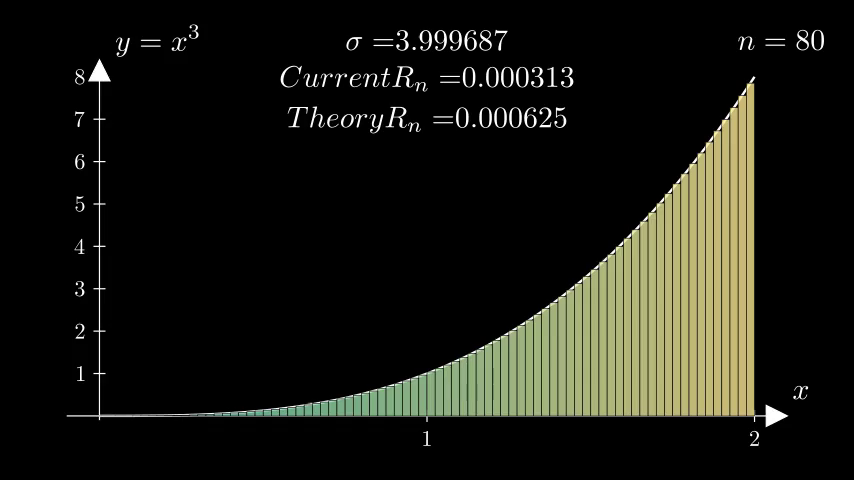
\includegraphics[width=\linewidth]{"./80.png"}
				\caption{при $n=80$}
			\end{subfigure}
			\begin{subfigure}{0.45\linewidth}
				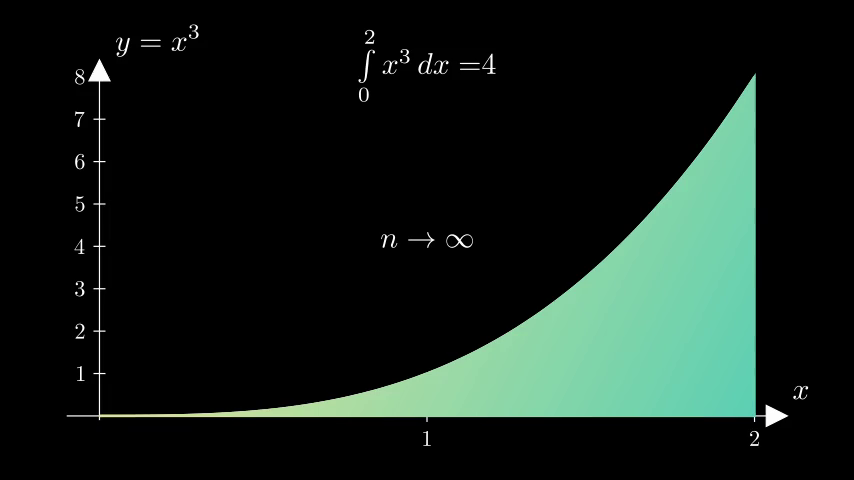
\includegraphics[width=\linewidth]{"./full.png"}
				\caption{при $n\to\infty$}
			\end{subfigure}
		\caption{Результаты работы программы при различных $n$}\label{result}
		\end{center}
	\end{figure}
\end{document}
